% Introduction
This section describes the application layer which takes advantage of the data stack described. The software described is the Hopsworks Feature Store, which this project contributes to.

\subsection{MLOps fundamental concepts}

\gls{MLOps} are a set of practices to automate and simplify \gls{ML} workflows from the data collection, to the model deployment. \gls{MLOps} considers the problem of developing and deploying a \gls{ML} system from a code point of view and data point of view. While for a typical software application, only code needs versioning, for a \gls{ML} application also data needs versioning, as training on different data versions might affect performance. The need for data versioning saw Feature Store emerge as a solution for the problem \cite{MeetMichelangeloUbers2017}. Feature stores play a central role in the \gls{MLOps} process, serving as fast-access storage during the process.

Figure \ref{fig:mlops} shows a simple \gls{MLOps} architecture making use of the Hopsworks' AI data platform. After data is gathered from various sources, a feature pipeline processes the data performing model-independent transformations and saving the resulting features in the Feature store. The training pipeline then runs model-dependent transformation (based on the specific model that is going to be trained), on the same features retrieved from the Feature Store and saves the output, i.e. the model in a Model registry. Then a last process is responsible for performing inference, and it is typically embedded in deployed applications. For this process, it will be enough to take the new features gathered on the platform and perform an inference on the specific model saved in the Model registry.

This type of architecture allows an asynchronous decoupled pipeline that enables the system to be maintainable, scalable, and extremely effective for production scenarios.

\begin{figure}[!ht]
    \begin{center}
      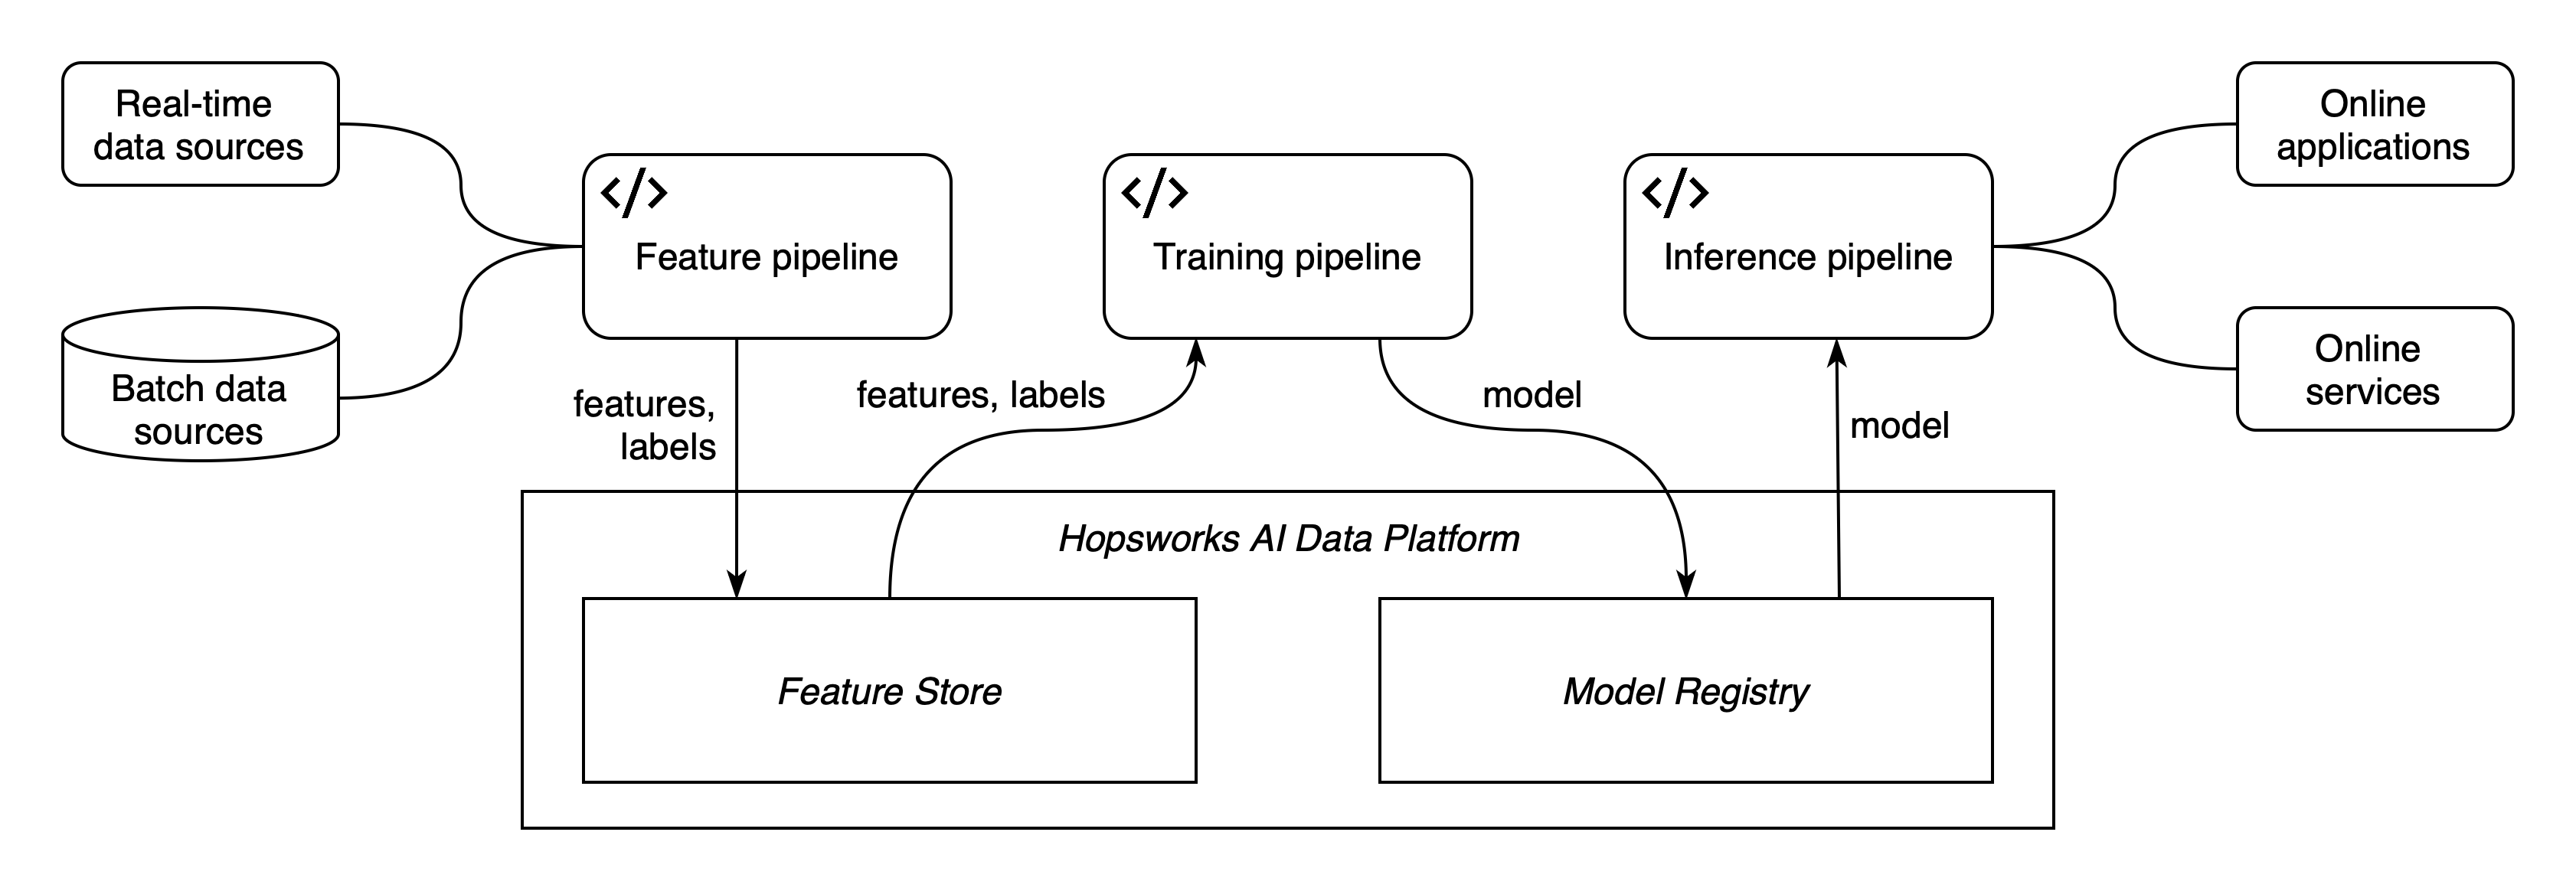
\includegraphics[width=\textwidth]{figures/2-background/MLOps.png}
    \end{center}
    \caption{\glstext{MLOps} pipeline using a Feature Store and a Model Registry}
    \label{fig:mlops}
\end{figure}


\subsection{Hopsworks Feature Store}

As first introduced in the previous section, the Feature Store is a key data layer in an \gls{MLOps} workflow. Feature Store enables feature reusability, a centralized and easier collaboration on model training and deployment. The Hopsworks Feature Store organizes features in feature groups, i.e. a mutable collection of features. Feature groups can be queried via the Hopsworks \gls{API} allowing developers to perform \gls{CRUD} operations.

The Hopsworks Feature Store in addition to supporting batch data sources also supports real-time data streaming. To be able to support both systems (or hybrids), the Hopsworks Feature Store saves features in two storages: the Offline Feature Store and the Online Feature Store. The Offline feature store is a column-based storage suited for batch data, that is updated with a low frequency (every few hours at maximum frequency). The Online feature store on the other hand is a row-based, key-value, data storage based on RonDB \cite{LogicalclocksRondb2024}. These characteristics enable low latency and real-time (in seconds) data processing. To keep this dual system consistent the Hopsworks Feature Store has a unique point of entry for data which is Kafka, that guarantees at least one message delivery to both storages. This enables the system to support both workflows while keeping consistent data storage.